\documentclass[letterpaper,12pt,twocolumn]{article}
\pagestyle{empty}

\pdfpagewidth 8.5in
\pdfpageheight 11in

\hoffset = 0pt
\oddsidemargin = 0pt
\marginparwidth = 0pt

\voffset = 0pt
\topmargin = 0pt
\headheight = 0pt
\headsep = 12pt

\textwidth = 7in
\textheight = 9.5in
\footskip = 0pt

\usepackage{amsmath}
\usepackage{amssymb}
\usepackage{hyperref}
\usepackage{graphicx}

\author{Erik Keever}
\title{Imogen User's Manual}

\begin{document} 

\maketitle

\section{Setup}

This section will guide you through the Imogen acquisition and setup process.

The setup process consists in making sure that you have the proper libraries
available and informing Imogen of where they are through the Make.config file
in the top level directory. The template Make.config.default should be copied
to Make.config and then setup per instructions below.

\subsection{Download}

Imogen lives online at \url{https://github.com/imogenproject/gpuImogen}

To download it into directory \textit{./gpuimogen} from the public repo,

\textit{ git clone https://github.com/imogenproject/gpuImogen.git ./gpuimogen }

\subsection{Matlab}

Imogen runs in Matlab and so obviously Matlab is a prerequisite to have. A standard
Matlab installation will have everything you need - the parallel computing toolkit
is not needed.

The \textit{MATLAB\_DIR} variable in Make.config must be set to the root of
the Matlab installation (e.g. /opt/Matlab/R2013b). Running Imogen in a different
Matlab version than used here to compile the binary modules is less likely than
might be imagined to cause problems.

\subsection{MPI}

MPI, even if parallel processing is not used, must be available (Imogen still
uses MPI to check that it is running serially), including development headers
to compile the Matlab mex files.

In Make.config, \textit{MPI\_DIR} must refer to the directory containing the include/ folder
that holds the mpi.h file, i.e. the --prefix specified when MPI was installed.

\subsection{Parallel Gateway}

Imogen uses the Parallel Gateway (PGW) library as a go-between with MPI.

Make.config's \textit{PGW\_DIR} variable must be set to the install directory
containing PGW.

\subsection{CUDA}

Imogen's GPU routines are written in CUDA and access to cuda 4.0 or later
libraries is required. The runtime alone isn't sufficient, the SDK is
needed to provide the headers.

Once it is installed set \textit{CUDA\_DIR} to the install location.

Other variables to be set are
\begin{itemize}
\item \textit{CUDA\_LDIR} - either 'lib' on 32bit or 'lib64' on 64bit machines
\item \textit{NVARCH} - \textit{compute\_20} for Fermi, \textit{compute\_30} for Kepler
\item \textit{NVCODE} - \textit{sm\_20} for Fermi, \textit{sm\_30} for Kepler
\end{itemize}

NVARCH and NVCODE are further explained by the nvcc manual page.

\subsection{Compiling}

Once all the above variables are set, run \textit{make} in both the mpi/ and gpuclass/
directories. Both build in parallel so feel free to use -j. 

\subsection{Filesystem}

Imogen will open/create the directory ~/Results. It is not required that this
be a shared filesystem.

\subsection{Cluster access}

Imogen invokes itself in parallel with the './imogen cluster ...' format.

This takes place on lines 95 to 124 of the run/imogen file. Before running
in parallel on a cluster it would be a good idea to examine this section since
it will almost certainly need to be amended, if only to set the package
names to their local values.

\subsection{Troubleshooting}

It is very important that PGW, MPI and the CUDA modules all be compiled
using the same compiler. PGW in particular is insistent about the version
of libfortran it accesses.

Unfortunately this is growing progressively more difficult as CUDA requires
newer GCCs and Mathworks' MEX compiler-wrapper lags.

If Imogen fails because Matlab complains about being unable to resolve an MPI
symbol, the problem is that Matlab defaults to lazy symbol resolution when
loading dynamic libraries and apparently something about the MPI lib trips
up on this. The solution:
\begin{itemize} \item LD\_PRELOAD="\$MPIDIR/lib/libmpi.so"
\end{itemize}
Putting this in your .bashrc (or as sysadmin, in the system's /etc/profile.d) will
make it go away permanently.

\section{Invocation}

Imogen is run through the script run/imogen

There are three separate general types of run:
\begin{itemize}
\item serial - One process uses ones GPU; Directly executed by script
\item parallel - N processes select N GPUs; Direct execution of mpirun by script
\item cluster - N processes on M nodes; Writes script and qsubs it
\end{itemize}

Serial and parallel are for small size simulations that work on a single SMP system,
while the cluster option uses qsub to fire jobs onto large systems.

The invocation syntaxes (also available through ./imogen -help) is as follows:
\begin{itemize}
\item ./imogen serial runfile.m [stream\# [GPU\#]];
\item ./imogen runfile.m; A shortcut that assumes serial, stream 0 and GPU 0.
\item ./imogen parallel runfile.m [stream\#] [NP]
\end{itemize}

\section{Selftest}

\textbf{This is not yet complete -- Erik}

Imogen includes a comprehensive full-simulation test, the simulation
\textit{run\_FullTestSuite.m}. This ``simulation'' will run dozens of test cases
for which an exact solution (or reasonable facimile thereof) is available
and determine whether Imogen is going them right and, where analytic answers
are available, provide convergence orders.

Note that there are a lot of tests to run, and this test falls under the "go have
lunch then check back" class.

\section{Physics}

\section{CFD}

At its core Imogen solves the Euler equations,

(insert Euler equations here)

using an adiabatic equation of state,

\[ eos \]

\textbf{This has been pretty thoroughly tested and should have no code problems.}

\subsection{MHD}

Imogen can simulate magnetic fields in the limit of Ideal MHD where the Euler equations
become:

(ideal mhd equations)

\subsection{Frame rotation}

In many cases a simulation is desired of an object that exhibits coherent rotation at
near-supersonic or (in e.g. the case of cold accretion disks) highly supersonic speeds.

By giving the center and rate of rotation Imogen allows the frame to be set in motion.
Reducing the grid-relative velocities means less risk of truncation error in the equation
of state, shorter simulation time due to reduced grid relative velocities and better
simulations due to reduced numerical diffusion (due to fewer steps).

This is controlled by setting the .frameRotateCenter and .frameRotateOmega parameters

FIXME: Imogen itself should take care of putting the simulation into the rotating frame
or at least offer the option. Currently the user is required to subtract off the momentum
associated with the frame's rotation in their own simulation init code...

\textbf{This has been tested using the Centrifuge experiment and appears to work properly.
Confidence is fairly high.}

\subsection{Radiation}

Imogen provides for radiative losses in the optically thin regime. The built in default
is power law cooling,

(power law lambda)

Programming in different cooling laws is extremely simple as a test by making additional
entries to the experiment/Radiation.m file, templatted after the thin power law radiation
one. Of course, don't expect them to be as fast as the GPU accelerated routines.

\textbf{Power law optically thin cooling should be completely reliable.} 

\subsection{Gravity}

\subsubsection{Point gravity}

Imogen allows the addition of massive points to the fluid simulation which obey Newton's
laws. Both point-point and point-fluid gravitational force are computed.

These points, ``compact objects'' as Imogen calls them, are used as standins for stars
or planets which cannot be resolved at reasonably available levels of resolution.

Far away from the object, they behave as point masses. Within a distance defined as
its 'radius', matter is considered as having been accreted. Each step, the mass and
linear and angular momentum in cells whose center is within r of a compact mass
are added to the compact object and replaced with grid's vaccuum values instead.

NOTE: This is not the desired behavior in some cases - e.g. a planet would require a surface
pressure, not a surface vaccuum, in order to be embedded in the disk.

\textbf{Point <-> disk gravity appears to work. Confidence is moderate pending testing.}

\subsubsection{Self gravity}

This is basically dead for now, especially in parallel.

The serial solver could easily enough be resurrected but there's no way I'm going
to have time to setup a parallel Poisson solver, let alone shovel it onto the GPU.

\section{Experiments}



\subsection{Centrifuge Test}

The centrifuge test checks the ability of the code to evolve an analytically time-independent
hydrodynamic flow and maintain its original time-independent values, and also provides a
valuable test of the rotating frame's implementation.

\subsubsection{Analysis}

The centrifuge test balances centripetal acceleration against a pressure gradient,
\[ \rho r \omega(r)^2 = dP/dr \]
Under the ideal gas law,
\[ P = K \rho T \]
and assuming that we are dealing with a thermodynamically simple gas or mixture whose 
internal degrees of freedom are pleasantly unchanging,
\[ \rho r \omega(r)^2 = K T d\rho/dr + K \rho dT/dr \]

Two of $\omega$, $\rho$ and $T$ have to be specified, then our differential equation
plus boundary conditions defines the third.

We chose to define an arbitrary $\omega$, except for the requirement that velocity behave
itself at the origin (diverging slower than $1/r$) and that $\omega$ is defined on a
compact region $[0, r_0]$, outside of which it equals zero (in other words, fluid at rest
at infinity).

Isobaric conditions are impossible, but isothermal, isochoric and adiabatic equilibria
can all be defined for any sane initial conditions. The ODE is solved by separation
of variables; Because it occurs often, the quantity
\[ \int_{r_0}^r r \omega(r)^2 dr \equiv \Phi(r,r0) \]
to save space.

\textbf{Isothermal}
With a fixed temperature (represented in the code as a fixed isothermal soundspeed), the ODE
\[ \Phi(r,r_0) = K T \int_{\rho_0}^\rho d\rho / \rho \]
is separated and has solution
\[ \rho(r)  = \rho_0 e^{\Phi(r,r_0)/KT} \]
With $\rho_0$ specified at the outer edge radius $r_0$ and an isothermal soundspeed $KT$,
a physical solution exists for sane inputs.

\textbf{Isochoric}
At a fixed volume (here taken as fixed density), the ODE
\[ \Phi(r,r_0) = K \int_{T_0}^T dT \]
is separated and has solution
\[ T(r) = (a^2 + \Phi(r,r0))/K \]
which gives pressure
\[ P = \rho K T = \rho_0 (a^2 + \Phi(r,r0)) \]
With the initial temperature set by proxy by isothermal soundspeed $a$ at the center
and density fixed, the temperature ramps up as required and a solution exists for sane
inputs.

\textbf{Adiabatic}
Under adiabatic conditions we use the relation $P = K \rho^\gamma$ and so
\[ \frac{\Phi(r,r_0)}{K \gamma} = \int_{\rho_0}^\rho \rho^{\gamma-2} d\rho \]
with solution
\[ \rho(r) = \left[ \rho_0^{\gamma-1} + \frac{(\gamma-1)\Phi(r,r_0)}{K \gamma} \right]^{1/(\gamma-1)} \]
Defining $\rho_0$ at $r_0$ and given $K$, a solution exists for all sane inputs.

\subsubsection{Initial Conditions}

The physical input parameters to the centifuge test are:
\begin{itemize}
\item \tt{rho0}
\item \tt{polyK}
\item \tt{cs0}
\item \tt{omegaCurve} is an anonymous function of an array $r$ which gives $\omega(r)$. This is assumed to obey the constraints given. $r$ is normalized between 0 (center) and 1 (edge).
\item \tt{eqnOfState} must be symbolically set to one of the \tt{CentrifugeInitializer} class' symbolic values \tt{EOS\_ISOTHERMAL}, \tt{EOS\_ISOCHORIC} or \tt{EOS\_ADIABATIC}.
\end{itemize}

Two additional numeric parameters are
\begin{itemize}
\item \tt{edgeFraction} - Sets how far the simulation domain extends past the edge of the
rotating region
\item \tt{omega0} - Sets the rate at which the simulation frame is rotated. This can improve the timestep considerably if rotation is in one direction and advection speed dominates soundspeed.
\end{itemize}

with the initial conditions set by
\begin{align*}
\rho(x,y,z) &= \rho_0(r) \\
\mathbf{v(x,y,z)} &= r (\omega(r) - \omega_0) \hat{\phi} \\
P &= P_0(r)
\end{align*}
the simulation proceeds adiabatically with the set index $\gamma$.

 



\subsection{Double Blast Test}

Two interacting blast waves on a 1-dimensional grid. This test is very difficult to solve on an Eulerian grid due to the 
strong shocks and multiple interactions with rarefactions and contact discontinuities, and is useful in measuring a 
solver's ability to handle these types of events. 

\subsubsection{Analysis}

The two blast waves propogate toward one another and collide, producing more contact discontinuities.
Could calculate the exact time they collide. Solve sod problem.

\begin{figure*}
\begin{center}
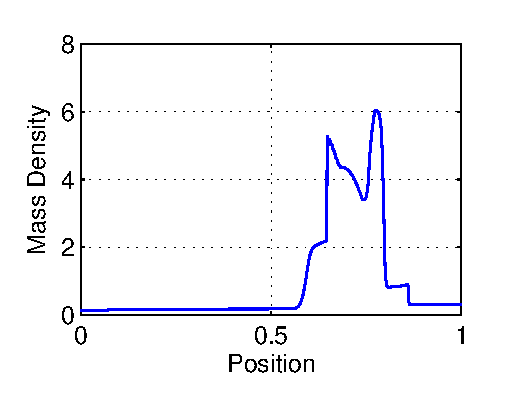
\includegraphics{DoubleBlast.eps}
\caption{Double Blast at t = 0.038}
\end{center}
\end{figure*}
\subsubsection{Initial Conditions}

Boundary conditions are mirrored around the X axis and periodic everywhere else.

The physical input parameters to the double blast test are:
\begin{itemize}
\item \tt{Pl} - Sets the pressure of the blastwave originating in the left-most tenth of the grid
\item \tt{Pr} - Similarly sets the pressure of the right-most blastwave
\item \tt{Pa} - Sets the ambient pressure
\end{itemize}


with the initial conditions set by each of the three zones being defined as an adiabatic gas with $\gamma$ = 1.4 everywhere. 
We set $\tt{Pl} = 1000$, $\tt{Pr} = 100$, and $\tt{Pa} = 0.01$. Initial momenta are zero everywhere.



\subsection{Einfeldt Strong Rarefaction Test}

This test measures the solver's vulnerability to very strong rarefactions that can, in some cases, 
produce negative mass densities or pressures. The input parameters can be tweaked slowly to determine 
exactly how strong the rarefaction can become before producing values that are NAN. 

\subsubsection{Analysis}

\subsubsection{Initial Conditions}

Einfeldt's Strong Rarefaction test consists of a 1-dimensional grid divided exactly in half. The 
properties of each half are defined separately, using four physical parameters. When run, the test 
produces two strong rarefaction waves moving away from the midpoint of the grid.

The physical input parameters to the Einfeldt Strong Rarefaction test are:
\begin{itemize}
\item \tt{rho} - Defines the mass density of the region
\item \tt{m} - Defines the X-momentum of the region (parallel to the grid)
\item \tt{n} - Defines the Y-momentum of the region (perpendicular to the grid)
\item \tt{e} - Defines the energy density of the region
\end{itemize}

The four parameters are saved separately as rhol and rhor, ml and mr, and so on.



\subsection{Richtmyer-Meshkov Instability Test}

RMI occurs whenever a plane shockwave becomes incident upon a non-uniform density interface. 
The plane shock refracts through the interface, imparting differential vorticity that drives
a jet from the denser fluid into the lighter fluid.

\subsubsection{Analysis}

For this run, we used a square grid 2048 zones across, for 20,000 iterations.
\begin{figure*}
\begin{center}
\includegraphics[width=.5\textwidth]{RMI.eps}
\caption{Richtmyer-Meshkov instability at t = 6504}
\end{center}
\end{figure*}

\subsubsection{Initial Conditions}
Boundary conditions are periodic around the X axis, constant around the Y axis, and mirrored around the Z axis.

The physical input parameters to the Richtmyer-Meshkov Instability test are:
\begin{itemize}
\item \tt{mach} - Defines the mach speed of the incoming shock wave
\item \tt{rhotop} - Defines the density of the lighter fluid 
\item \tt{rhobottom} - Defines the density of the heavier fluid
\end{itemize}

To create the non-uniform interface, we create a cosine wave with an amplitude 1/20 of the height 
of the grid and with a wavelength 2x the length of the grid. We then place the center of the wave 
4 total wave amplitudes below the center of the grid, and set the mass density of the entire 
region below the wave equal to rhobottom. The rest of the grid is previously set to have density 
equal to rhotop, and is unchanged by the wave. We then create a shocked region from the top of 
the grid to a height just 20 zones above the peak of the wave. This shock is composed of a momentum 
and pressure equal to a blast wave with mach set by the input 'mach'.

Note that the entire region must then be given a momentum in the direction opposing the shock to 
maintain position on the grid. This opposing momentum is calculated by the same function as is used 
to calculate the initial shock.



\end{document}
